\documentclass[11pt]{article}
%\renewcommand{\familydefault}{\ttdefault}
%Some packages I commonly use.
\usepackage{blindtext}
\usepackage[T1]{fontenc}
\usepackage[english]{babel}
\usepackage{mathptmx}
%\usepackage{graphicx}
%\usepackage{framed}
%\usepackage[normalem]{ulem}
%\usepackage{amsmath}
%\usepackage{amsthm}
%\usepackage{amssymb}
%\usepackage{amsfonts}
%\usepackage{enumerate}
\usepackage[utf8]{inputenc}
\usepackage[top=1 in,bottom=1in, left=1 in, right=1 in]{geometry}
\usepackage{amsmath}
\usepackage{mathrsfs}
\usepackage{amssymb}
\usepackage{graphicx}
\usepackage[colorinlistoftodos]{todonotes}
\usepackage[colorlinks=true, allcolors=blue]{hyperref}
\usepackage{listings}
\providecommand{\keywords}[1]{\textbf{\textit{Keywords---}} #1}
%\usepackage{flafter}
\usepackage{float}
%\usepackage{enumitem}
%\usepackage{varwidth}
%\usepackage{natbib}
% Please add the following required packages to your document preamble:
%\usepackage[normalem]{ulem}
%\usepackage{todonotes}
%\useunder{\uline}{\ul}{}


%A bunch of definitions that make my life easier
\newcommand{\todoF}[2][]{\todo[color=red!25, #1]{#2}}
\newcommand{\todoINFO}[1]{\todo[color=blue!25]{INFO: #1}}
\newcommand{\todoIMPORTANT}[1]{\todo[color=red!25]{IMPORTANT: #1}}
\newcommand{\todoREV}[1]{\todo[color=green!25]{REVIEWED: #1}}







\title{A Survey of Interactive Theorem Proving Systems and Their Practical Aspects in Large-Scale Formal Verification }
\author{Fariba Khan  \\
	School of EECS \\
	Oregon State University \\
	khanfari@oregonstate.edu
}
\date{}


\begin{document}
	
	
\maketitle

\begin{abstract}
	
Interactive theorem proving (ITP) systems let human and machine work together to build machine-checked formal proofs. Different ITP systems has emerged following different formal foundations of mathematics with their own set of interesting features. These systems are now being widely used in formal verification of large-scale complex systems to increase their reliability, leading to equally large-scale proof development. Consequently, the focus of proof assistant research has been expanded to practical aspects of ITP systems to identify and address domain-specific challenges in large-scale development. This survey organizes existing research on these practical aspects, along with a brief overview of interactive theorem proving systems themselves. It also draws attention to significant challenges and open problems identified by the researchers across literature.\\

\keywords{Proof Assistants, Interactive Theorem Proving, Proof Engineering, Large Scale Verification, Formalization,
	Formal Verification, Proof Development, Proof Maintenance, Proof Refactoring, Proof Repair, Proof Robustness, Usability.}
	
\end{abstract}



\section{Introduction}
\label{sec:intro}

In recent years, interactive theorem proving (ITP) that assists humans in the intriguing task of building formal machine-checked proofs, has been emerging in the formidable area of large-scale complex system formal verification, leading to new challenges in proof development and maintenance. In theorem proving, the goal of proofs is to validate the correctness of a mathematical statement. Any mathematical proof can be spelled out into simple steps that can be verified irrefutably, and this is the main idea behind the machine checking of proofs. Proofs need to be translated from informal language to formal language i.e. formal system, where each proof step is either an axiom of the formal system or can be inferred from one through its valid inference rules. However, in the interactive arrangement, the machine's role is not only to check whether a human written proof i.e., proof script, is valid in some formal system but, more importantly, to assist in finding that valid formal proof. Different formal systems have prompted the development of different interactive theorem proving systems, also known as proof assistants, who play this role of machine. However, formalization of a system is different from the formalization in mathematics in the sense that it entails more than just the aforementioned translation. One needs to identify the system's properties that ensure its correctness before going about translating them into formal statements and finding corresponding proofs. Intricacy and scale of the set of properties reflect the complexity and size of the underlying system, and specification of these properties often evolves with the system as well. With the increasing formal verification of the large-scale complex system in proof assistants following successful ventures like verified C compiler CompCert C~\cite{Leroy_2006}, proof development is now getting scaled at an unprecedented rate. Therefore, proof development too calls for methodologies to facilitate efficiency and maintainability i.e., proof engineering, just like efficient software development demands for software engineering. These proof engineering aspects of proof development in ITP systems are considered as practical aspects of proof assistants in this survey. Some impressive works have already been done by researchers to identify challenges in large-scale system verification along with efficient methodologies to handle them. Still, proof engineering is far away from reaching the maturity level of software engineering. This survey presents existing research on practical aspects of ITP systems in large-scale system verification by categorizing them with respect to the proof engineering concerns they address i.e., identifying the challenges and requirements in large-scale system verification (Section~\ref{sec:ITPinLarge}), providing methodologies for efficient development of maintainable proofs (Section~\ref{sec:proofDev}), aiding in maintenance of existing proofs over time through automated techniques (Section~\ref{sec:maintenance}), supporting development through tooling and Integrated Development Environment (IDE) from ITP systems (Section~\ref{sec:tooling}). However, before diving into research on practical aspects, this survey provides an overview of the ITP systems to acquaint readers with salient characteristics of different systems (Section~\ref{sec:overview}). Throughout the survey, it also points out the difference among ITP systems both in terms of their features and their practical aspects, as well as draws attention to significant challenges and open problems identified by the researchers.

%which is essential to understand the techniques presented in the literature
%Still, proof engineering is far away from reaching the maturity level of software engineering. In this survey, I am going to present existing research on practical aspects of ITP systems in large-scale development by categorizing them with respect to the proof engineering concerns they address i.e., i.e. identifying the challenges and requirements in large-scale development (Section ~\ref{sec:ITPinLarge}) and then, finding methodologies and  to tackle them. These methods and techniques across literature can further be categorized into two categories - a) proactive measures to be followed during proof creation to facilitate efficient development of maintainable proofs (Section ~\ref{sec:proofDev}), and b) reactive measures to be applied over time to adapt existing proofs to changes(Section ~\ref{sec:maintenance}). 

%Finding challenges and requirements for large scale development  These challenges and the requirements for large scale development will be discussed in section~\ref{sec:ITPinLarge}. Methodologies to tackle these challenges can further be categorized into proactive measures to be followed during proof design and development and reactive measures to   i.e. identifying the challenges and requirements in large-scale system verification (Section ~\ref{sec:ITPinLarge}), providing design methodologies for efficient development of maintainable proofs (Section ~\ref{sec:proofDev}), aiding in maintenance of proofs over time through automated techniques (Section ~\ref{sec:maintenance}), supporting development through tooling and IDE from ITP system (Section ~\ref{sec:tooling}). However, before diving into research on practical aspects, I will provide an overview of the ITP systems and their salient characteristics (Section ~\ref{sec:overview}), which is essential to understand the aforementioned techniques presented in the literature. This whole survey will also attempt to point out the difference among ITP systems both in terms of their features and their practical aspects, as well as will try draw attention to significant challenges and open problems identified by the researchers.

%Still, proof engineering is far away from reaching the maturity level of software engineering. In this survey, I am going to present existing research on practical aspects of ITP systems in large-scale development by categorizing them with respect to the proof engineering concerns they address. Identifying challenges and requirements for large scale development will be discussed in Section~\ref{sec:ITPinLarge}.    i.e. identifying the challenges and requirements in large-scale system verification (Section ~\ref{sec:ITPinLarge}), providing design methodologies for efficient development of maintainable proofs (Section ~\ref{sec:proofDev}), aiding in maintenance of proofs over time through automated techniques (Section ~\ref{sec:maintenance}), supporting development through tooling and IDE from ITP system (Section ~\ref{sec:tooling}). However, before diving into research on practical aspects, I will provide an overview of the ITP systems and their salient characteristics (Section ~\ref{sec:overview}), which is essential to understand the aforementioned techniques presented in the literature. This whole survey will also attempt to point out the difference among ITP systems both in terms of their features and their practical aspects, as well as will try draw attention to significant challenges and open problems identified by the researchers.

%through formalization
%in the readers need an introduction to the ITP systems and their characteristics to understand the techniques presented on the 
%Different interactive theorem proving systems, also known as proof assistants, has been developed with the emergence of different formal systems.
%Nevertheless, to reach the maturity level of software engineering, researchers need to find and address open challenges
%with the help of some proof assistant




 %intro
\section{Overview of Interaction Theorem Proving (ITP) Systems}
\label{sec:overview}

This section provides a brief overview of the ITP systems in terms of their major distinguishing characteristics followed by a detailed comparison of a small set of representative systems. Although the focus of this survey is not on the formal logic underlying the proof assistants, to understand the difference among them as well as the techniques from the literature described in later sections, we need to talk about theories at least to some extent. In fact, salient characteristics that distinguish different ITP systems boost from the formal foundations they are based on. In the following, these ITP systems are introduced as they historically emerged following the development of the different formal foundations of mathematics informing readers to both simultaneously. % in an attempt to familiarize readers simultaneously to both.

The first attempt in mechanical verification of mathematical proofs is the Automath~\cite{Bruijn_1983} system, initiated by De Bruijn in 1967. It treats proof as a first-class object like any other term in formal language. This technique, in logic, is known as Curry-Howard-Isomorphism that states one-to-one correspondence between formal proof calculi and type systems for a model of computation, e.g., between natural deduction and typed system for lambda calculus. %This correspondence, in fact, splits into two - formula_as_types and proof_as_programs. 
Martin-L{\"o}f’s Intuitionistic Theory of Types~\cite{Lof_1984} extends the Curry-Howard-Isomorphism to predicate logic by introducing dependent types and then later, after the discovery of Girad's paradox, replaced the original impredicative version with a consistent predicative version. There are both extensional and intensional variants of this type theory, which are implemented in proof assistants Nuprl and Agda, respectively. I'll explain both predicativity and intensionality later in the section. 

On the other hand, under Curry-Howard-Isomorphism, Girad's polymorphic $\lambda$-calculus, system F\_$\omega$, corresponds to higher-order logic. Theory Coquand, in 1985, combined system F\_$\omega$ with impredicative Martin-L{\"o}f type theory in a higher-order extension of Automath language and presented Calculus of Constructions (CoC)~\cite{Coquand_Huet_1988}. CoC was later extended with primitive inductive extension leading to the Calculus of Inductive Constructions (CIC). The proof assistant, Coq, is the implementation of this calculus. The current Coq system's logic is dependently typed, higher-order, partially predicative, and intensional~\cite{Coq_2019}.

Automath also initiated the concept of Logical Framework. De Bruijn's systems only give basic mathematical mechanisms and let the user implement their preferred logical rules. Thus, in a logical framework, one can embed a logic as a signature in the framework's type theory, and the provability of a formula in the embedded logic comes down to the type inhabitation problem of the framework's type theory. Systems LF, Twelf are some implementations of Logical framework. Around the same time as Automath, another deductive system, the logic of computable functions was devised by Dana Scott~\cite{Scott_1993} and later, implemented in an ITP system, called Logic for Computable Functions (LCF), by Robin Milner and his collaborators at Stanford, Edinburgh, and Cambridge. Milner later developed the \emph{LCF approach} for his systems to not to require storing and rechecking of large proof objects~\cite{Geuvers_2009}. This LCF approach provides soundness by construction by making proofs terms of an abstract data type \emph{thm} whose predefined values are axioms and constructors are primitive inference rules of the logic. One can only create a term of \emph{thm} via the inference rules; thus, the proof has to be sound. Several present ITP systems, including as Isabelle~\cite{Wenzel_2008}, HOL~\cite{Gordon_Melham_1993}, and HOL-Light, are successors of LCF system. Isabelle, in fact, is an LCF style logical framework with the logic directly encoded in LCF style serving as meta-logic for other logic to be embedded as object logic. Examples of embedding are Isabelle/HOL and Isabelle/ZF, where HOL is classical higher-order object logic, and ZF stands for first-order Zermelo-Frankel set theory. 

There are few other active ITP systems that have not been mentioned above. Among them, Mizar is quite notable for its largest repository of formalized mathematics called the Mizar Mathematical Library (MML). Mizar's other famous and influential feature is its declarative input language, which enables batch proof checking. It can check a whole file at once even if there are some proof steps not acceptable by the solver, consequently creating a syntactically correct proof with potential holes in it. The precise notion of this method can be found in Wiedijk's work~\cite{Wiedijk_2003_b}. This feature, named Mizar Mode, has been incorporated in many proof assistants, including HOL, HOL Light, Isabelle, Coq~\cite{Geuvers_2009, ringer_et_al_2019_b}. A complete overview of all other ITP systems such as LEGO, Lean, Idris can be found in~\cite{Wiedijk_2003_a, Harrison_2014, Geuvers_2009}.

\subsection{Detailed Comparison of a Few ITP Systems}

For the detailed comparison, I have selected the representative systems Coq, Agda, Nuprl, Isabelle/HOL in the attempt to cover most formal systems and their branches. They are compared based on the following categories that have practical implications on proof development. \\

%to represent systems based on impredicative Calculus of Inductive Construction, Predicative Martin-L{\"o}f intensional, Predicative Martin-L{\"o}f extensional, intensional  

\textbf{Equality}
The definition of \emph{equality} in type theory has great implication on proof development and type checking in the corresponding proof assistant. Extensional and intensional type theories handle \emph{equality} differently. Extensional equality considers two objects to be equal if their external properties are alike i.e., they behave the same way with its environment. Intensional equality, on the other hand, requires the internal structure of the entities to be equal as well. For example, $f(n) = 3*n + 9$ and $g(n) = 3 * (n+3)$ are equal in extensional sense but not, in intensional sense. Similarly, two functions are considered equal by extensionality, known as \emph{function extensionality} if they produce same outputs for the same inputs, where in intensionality, their implementation needs to same as well. Therefore, in proof assistants, based on intensional type theory such as Coq, Agda, if inductive definition of plus (+) defines $0 + n = n$ but not $n + 0 = n$, then any statement of the later construct needs additional induction reasoning to hold i.e. needs to be proved. On the other hand, in extensional type theory based proof assistants such as Nuprl,type checking is undecidable. The reason is in extensional type theory, \emph{definitional equality} that refers to equality by construction, and \emph{propositional equality}, used in propositional statements to be proved, coincide. Consequently, undecidable programs can be specified in the type system making type checking undecidable. However, in intensional type theory \emph{definitional equality} and \emph{propositional equality} are completely distinct, and type checking is decidable. \\

\textbf{De Bruijn Criterion} 
De Bruijn Criterion~\cite{Barendregt_Geuvers_2001} requires proof assistants to produce an independently checkable proof object for the interactively created proof in the system. This proof object should be easily verified by skeptic users by writing a simple type checking algorithm. This is one of the four ways identified by H. Guevers~\cite{Geuvers_2009} to guarantee the correctness of ITP systems. Coq, Agda, Nuprl all meet the De Bruijn criterion. However, systems based on LCF, such as Isabelle, do not produce a complete proof object as each step is constructed with the guarantee that it is correct. In that sense, they do not meet the \emph{De Bruijn criterion} though it should not be hard to generate a proof object on the side if needed. The practical implication is that, in the LCF approach, there is no need to check the system with respect to the theory anymore as its inference rules and axioms are implemented directly to create the proof. \\

\textbf{Predicativity}
Predicativity of type theory has impact on its consistency as well as on its expressiveness. Impredicative refers to self-referential definition i.e., a definition that mentions or quantifies over itself. To be predicative, a definition can not mention itself, and if it contains quantifiers, then they can not be initiated with an object defined by the definition. Impredicative type system can be shown inconsistent by Girad's paradox thus Martin-L{\"o}f made his type theory predicative. Agda, Nuprl, meta-logic in Isabelle, all are predicative. However, in Coq, Type universe, including Set is predicative, but the Prop universe is still impredicative due to the informally agreed notion that it is often easier to express mathematical proofs with impredicativity. \\

\textbf{Termination and Totality}
In proof assistants based on intuitionistic type theories such as Coq, Agda, and Nuprl, functions need to be terminating for the logic to be consistent. Recursive calls have to be made on the subterm of the arguments to ensure their termination. For advanced cases where termination cannot be proven automatically, explicit proof of termination needs to be provided, or special approaches like exploiting the size of argument terms~\cite{Abel_et_al_2017, Ringer_et_al_2019} needs to be used. Agda provides induction-recursion that lets the user define mutually recursive functions and data types. Coq does not have this mechanism. However, classical higher-order logic in HOL, do not need a termination witness, but the use of the non-terminating function is limited~\cite{Ringer_et_al_2019}. Moreover, functions in HOL and CIC logic need to total, and partial function needs indirect encoding into the logic. These requirements are two difficulties beginners in ITP usually encounter, even if they are already familiar with functional programming language~\cite{Ringer_et_al_2019}. \\
%total partial~\cite{McBride 2015, Capretta, V. 2005, Bertot and Casteran, 2004, Ringer}

\textbf{Proof Creation Style}
Proof creation style varies widely among ITP systems. In Coq, although it supports forward style, the usual way to create a proof is to use backward style (top-down). The user keeps applying tactics to the current goal, which creates subgoals needed to be proven separately, until True is reached. Proof development in Nuprl also follows the top-down approach. However, in Isabelle, the usual way is the forward style (bottom-up), where proofs are created from axioms and inference rules from the logic. Proof context gets enriched by new facts keeping the goal same, until the goal is reached~\cite{Yushkovskiy_Tripakis_2018}. However, both of them support tactics and provide tactic languages Ltac and Eisbach, respectively, to allow writing custom tactics. They also have proof languages like Coq/SSReflect and Isabelle/Isar. Proof languages aid in writing understandable proofs inspired by mathematical vernacular, in contrast to unstructured sequences of tactics. Users can reconstruct an English proof just form the script of the proof instead of stepping through tactics and tracking goal transformation. 

However, in Agda, there is no support for the separate tactic language, although an automatic proof search tool, Agsy that works like \emph{auto} tactic in Coq is there. Agda's dependent types let the user write almost any proposition. Proofs can be written as the term of the type of its theorem proposition. However, users can build proofs interactively in Emacs or atoms by putting a question mark (?) in the place of an expression, usually the proof term they need to write. Agda is able to type check incomplete programs with holes, i.e. (?) marks and can provide a list of the context, infer the type of the expression at the hole, and even sometimes evaluate the open term if bound variables in surrounding context are provided. Agda, like Idris, is basically a dependently typed programming language whose type storing and dependent types let it act as a proof assistant. The syntax in Agda is Haskell like where Coq's syntax is ML like. \\

\textbf{Dependent Types and Pattern Matching on them} 
Coq, Agda, and Nuprl support dependent types, but Isabelle/HOL does not have dependent types. However, it is easier to pattern match on dependent types in Agda than in Coq. In coq, one needs to use complex clause like \emph{match.....as.....return} clauses for that. Examples of pattern matching on indexed datatypes in Coq and Agda are shown side by side in the following Fig~\ref{fig:overview_1}.  \\


\begin{figure}[H]
	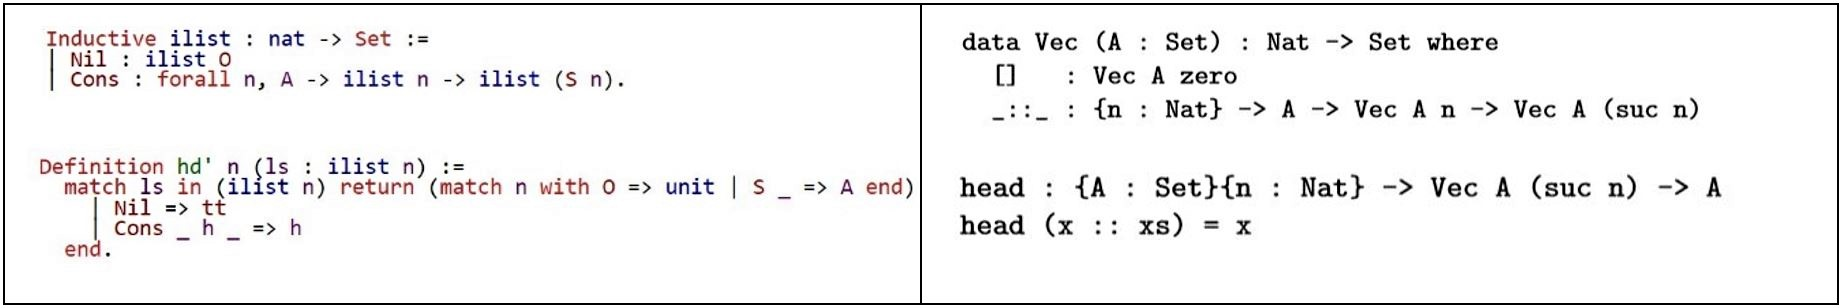
\includegraphics[width=15cm]{figures/fig_1.JPG}
	\centering
	\caption{Pattern matching on indexed data-types in Coq and Agda respectively~\cite{Chlipala_CPDT_2013}~\cite{Norell_2009}}
	\label{fig:overview_1}
\end{figure}


\textbf{Program Extraction}
Program extraction from proofs let certified program to be extracted and executed in favorable run-time environment.This mechanism is beneficial for system verification projects. Coq supports the extraction of executable programs in Ocaml and Haskell from proofs. Agda does not have any such support at this moment. Isabelle/HOL also has a code generation scheme based on the work of Haftmann and Nipkow~\cite{Haftmann_Nipkow_2010}. It translates HOL to an intermediate language called Mini-Haskell and then, translates from this Mini-Haskell to Ocaml, Haskell or Standard ML. \\

\textbf{Classical axioms}
Classical axioms cannot be proved in all proof assistants because of their underlying logic, thus require special techniques when they are needed in proof development but not supported by the ITP systems. Isabelle/HOL is based on classical higher-order logic. Hence, all classical axioms, e.g., Excluded middle, Double negations, are valid here. However, in intuitionistic logic, not all of them hold. For example, the double negation introduction law can be easily proven in intuitionistic logic, but neither the double negation elimination rule nor the Excluded middle can be proven. One way to embed Excluded middle axiom into intuitionistic logic is by double negating it, which is known as Glivenko's double-negation translation. Other classical axioms can also be translated through various translations such as Kudro's translation, G{\"o}del-Gentzen translation~\cite{Yushkovskiy_Tripakis_2018}. Coq provides a library, Coq.Logic.Classical\_Prop with classical axioms, to extend its intuitionistic logic to classical logic. 













 %overview
\section{Challenges in Large-Scale Formal Verification}
\label{sec:ITPinLarge}

One important application of iterative theorem proving systems is formal verification of large complex systems. An increasing number of large scale system verification projects has been carried out in recent decades and has appeared as published case studies in literature. One of the successfully commercialized verification projects is the certified C compiler, CompCert~\cite{Leroy_2006, Leroy_2009}, for which Leory's work~\cite{Leroy_2006} received the Test of the Time award in POPL (Symposium on Principles of Programming Languages) 2016 and was noted as a groundbreaking contribution in demonstrating the feasibility of interactive theorem prover~\cite{ACM_SIGPLAN_2016}. It's indeed a groundbreaking achievement even in terms of effort, given the scale of the project with 350,000 lines of Coq code along with state of the art of ITP systems at that time. Having tens of thousands of lines of code is not at all unusual in large proof development, irrespective of the ITP systems used in the project. Certification of seL4 Operating System Kernel by Klein \emph{et. al.}~\cite{Klein_et_al_2009} produced about 480,000 lines of code in Isabelle/HOL~\cite{Klein_et_al_2014}, Coq correctness proofs of an Raft distributed consensus protocol~\cite{Ongaro_et_al_2014} comprises of 50k lines in total~\cite{Woos_et_al_2016}. However, hurdles behind these verification works are not only due to the size. The biggest challenge comes from the complexity of the underlying system such as non-trivial concurrent OS kernel~\cite{Gu_et_al_2016}. Industrial design specification is often performance-oriented, thus imprecise in nature, which impedes the creation of clear and elegant abstract specifications needed for formal verification~\cite{Kaivola_et_al_2003}. Sometimes verification even gets carried out as part of an active, hence evolving development project. Interactive theorem proving is itself hard, and together with the issues mentioned above, it takes multiple persons years of effort for a single verification project~\cite{Delaware_et_al_2011}. Proof engineers and researchers involved in many of these large-scale projects later reported they could have saved lots of time if, from the beginning of proof development, they followed some schemes that facilitate adaptability, well-organization and reusability of proofs~\cite{Curzon_1995, Kaivola_et_al_2003, Woos_et_al_2016}. In fact, these attributes of proofs have been repeatedly identified by researchers that promote maintainability and efficiency i.e. the two main challenges in large scale development. Klein \emph{et. al.}~\cite{Klein_et_al_2014} also provides a picture of how often they needed to adapt their proofs to changes and how bad the maintenance cost was for that at the time of their sel4 OS kernel verification~\cite{Klein_et_al_2009}. 17\% of their total proof effort was just to reverify their system in response to fundamental changes in existing features of sel4 kernel. This is only one of the four kinds of changes they encountered. To be noted here, this verification project was carried out as part of the development of the kernel itself. 

Not surprisingly, many of these large projects were followed up with work on methodologies for maintainable and efficient development. Although these methodologies were initially devised to be used in their respective projects, in the follow-up papers, they tried to generalize their solutions to be used irrespective of domains\cite{Curzon_1995, Delaware_et_al_2011, Kaivola_et_al_2003, Woos_et_al_2016}. Apart from these, some notable works have been done on proof reusability. However, even with conscious attention to maintainability during proof design and development, some unforeseen or unpredictable changes are bound to happen. Adapting proofs in large scale development to these changes has been identified as another challenging aspect of large-scale proof engineering. Researcher have also begun working on refactoring and repairing techniques to incorporate these changes efficiently. Therefore, research on maintainability and efficiency issues of large-scale proof development can be categorized as proactive measures to be followed during proof design and development and reactive measures to adapt proofs to changes anytime. Following two sections address them respectively.

%these solutions are closely related to the associated project insinuated from the insight they gained from experience and difficulties they encountered during the development process, the general goal across these papers is to analyze and tackle issues associated with scaling~
%Apart from the works mentioned above on tackling issues with large scale development, there is also a substantial amount of impactful work in mechanizing metatheory. Proving properties of programming languages often need a different set of tools in ITPs such as the representation of binders or complex inductions ~\cite{Aydemir_et_al_2005}. 

%Key challenges in this domain identified by the POPLMark challenge are the representation of binders, complex inductions, experimentation, and reuse of components.

% ** In the following two sections, I am going to categorize the research on these practical aspects of theorem proving in two areas - a) design strategies to be followed during proof development both for scalability and mechanized metatheory, b) refactoring and repair techniques to handle changes over time. Then, I'll give a summary of the methods that have been integrated into tools or supported from the library level.

%From a high level perspective, proof engineering research can be categorized into two kinds - a) design strategies to be followed during proof development, b) refactoring and repair techniques to handle changes over time. 

%In the following sections, I am going to categorize the research on these practical aspects of theorem proving in two areas - strategies and framework for proof development and techniques and methods for proof maintenance over time. Then, I will give an overview of existing tooling and library level support for both of them.
%Some of these techniques are being integrated in tools as well.

%Apart from all these works on tackling issues with large scale development, there is one particular domain where interactive theorem has not only created a large practical impact also importance of application in that domain led to including features in ITPs' core language. As you have already guessed from the context or section title, I am talking about mechanized metathory. Some ideas from these domain can even be generalized to other domains. Considerable amount of influential works in this domain demonstrates practical aspects and impacts of ITPs, thus demands to be included in this survey. 

%Reflecting real systems and its properties accurately of paramount importance for the success of the task at hand.

%Without efficient strategies to facilitate proofs' adaptability, modifiability, robustness, reuse during proof development along with clever techniques to support its maintenance over time, interactive theorem proving would not be able to make as much impact as compared to its usefulness [describe usefulness in introduction]. Therefore, proof engineering research have been expanded to find methodologies and design principles handling the challenges in large scale development and some of these are being integrated in tools as well.
%[ don't need here: automation faciliates above feature : Moreover, a well-designed theorem along with attributes mentioned above should also make use of as much automation as required to keep programmer from reinventing the wheels and focusing on more complex parts that indeed require human guided strategy to solve.]
%Not surprisingly, a handful of  research that has been done on these aspects of proof engineering, was part or follow-up work of some large verification projects~\cite{}. Although these works stem from the experience of respective project concentrating on finding solution for the difficulties they faced during proof development stage, the general goal across these papers is to analyze and tackle issues associated with scaling. As a result, nearly all of these methods can be used irrespective of domains~\cite{woos 16, kaivola}. 
%However, there have been some works targeting issues in mechanizing metathory which demand specialized solutions like binder, ..... ~\cite{POPLmark challenge}. Here, I am limiting the scope of this work given the time constraint ignoring numerous other domain specialized methods in practice and even in mechanized metatheory only focusing research on framework for structuring. 
% In the following sections, I am going to categorize the research on these practical aspects of theorem proving in three areas - strategies and framework for proof development, techniques and methods for proof maintenance over time and existing tooling support for both of these aspects.
%\point {eg1: data evolution}
%\textbf{Context 1: schema evolution.}

%\emph{Every time the database evolves, a new ``variant'' is created.}

% The Mizar mathematical library is probably the most comprehensive formalization effort, but its declarative style makes it hard to employ proof search, and its source code is not freely available. Like Coq and HOL Light, also Isabelle [14] was used for major formalization efforts, such as the formalization of the seL4 microkernel [16]. We are not awareofacomprehensivecoverageoffundamentalmathematics in Isabelle, HOL4, or Lean. 
 %ITP in large scale
\section{Methodologies for Efficient and Maintainable Proof Development}
\label{sec:proofDev}


%Automation
%Organization (modularity, framework, compositionality )
%Abstraction
%Reuse (ornaments, combinators) 

%Formalization in large-scale demands for methodologies to make proof development process efficient or even feasible for complex systems. For a long time, mere proof creation rather than practical proof engineering for maintainability had been the primary concern of the Proof assistant designers~\cite{Curzon_1995}. However, recent advancement in large-scale verification has changed their perception. Large complex systems reap the benefit of formal verification the most, which in turn creates gigantic and complicated proof scripts. Also, proof development itself is an iterative process ~\cite{Woos_et_al_2016} and sometimes gets carried out as part of an active, hence evolving development project. Thus, f

Recent advancement in large-scale verification has expanded the focus of interactive theorem proving research from mere proof creation to practical proof engineering aspects~\cite{Curzon_1995}. Researchers are trying to come up with methodologies for designing well-organized and adaptable proofs to make development process efficient and maintainable~\cite{Kaivola_et_al_2003, Woos_et_al_2016, Curzon_1995}. The reusability of proofs also plays an essential role in promoting efficiency and maintainability. In the following two subsections, methodologies accumulated across literature are discussed under the two subcategories - a) methodologies for adaptability and organization, b) methodologies for reusability along with an account for how these strategies differ concerning ITP systems when applicable.

Moreover, proof engineers also benefit from some form of automation within the ITP as well as from the portability of proofs among different ITP systems to improve their performance, thereby efficiency of the overall proof development. A third subsection elaborates on gains from automation and portability as well as existing methods to facilitate them.

\subsection{Methodologies for Proof Organization and Adaptability}

%reason this way as adaptability facilitate efficiency
%Adaptability and maintainability go hand in hand. Proofs, to be well maintained, needs to be adaptable to changes. Unfortunately, interactively created proofs, although through hard-labor, can easily get broken in the face of changes and requires a substantial amount of time to recover, unless good design strategies are followed during proof creation. This brittle nature of proofs, together with the amount of required recovery work, has been identified as one of the major causes of inefficiency in many large proof developments (see section~\ref{sec:ITPinLarge} for references). 

Crafting robust, easily modifiable, strategically structured proofs play an important role in increasing efficiency during development. Features like modularity and abstractions in ITP systems, as well as custom or general-purpose tactics, can promote well organization and adaptability in proof development. \\

\textbf{Through Modularity and Abstraction} Modularity and abstraction can be used to write structured proofs. Organizing proof with good structuring principle often helps developers to compartmentalize their thoughts as well. For example, decomposing complex problems into simpler ones hierarchically based on their mutual dependencies lets the developer focus on one problem at a time. It also makes proving higher-level problems easier with already proved simpler ones they depend on. Software engineering has several methodologies for organizing and writing adaptable codes. Although these methods can give ideas for proof engineering, they often need to be improvised to be used in proof development. Information hiding from dependents or clients is one of these software development techniques, albeit a classic one. The trick here is one can not depend on the information they do not know, thus forcing dependents to write implementation without that information. This technique lets code to be updated without any changes to its clients. Proof engineering can also use this same technique by hiding functions' and types' definitions behind interfaces and reduce unnecessary rework. However, in proof development, dependents do not just use these definitions; they need to reason about them, which often demands more information. For instance, systems based on intensional type theory like CoQ depend on \emph{definitional equality}, thus needs detailed constructional information of function and types as well. Planning for change by Woos \emph{et. al.}~\cite{Woos_et_al_2016} addresses this problem by adding lemmas in the interface that are sufficient and necessary to reason about themselves while hiding the rest of the information. To be noted here, systems based on extensional type theory, like Nuprl, would not need these additional interface lemmas when reasoning for equality (see section~\ref{sec:overview} for detail). They also recommend using the interface to separate theorem statements from their proofs. This technique also leads to faster development. In proof assistants like Coq, checking after modifying one proof kicks off rechecking of all other proofs that depend on it. Thus, the developer needs to wait a while after each edit, and in a large development, 'a while' gets really long. Following the above recommendation, dependent proofs would only have to import interfaces containing statements. Unless interfaces are not modified, the rechecking of other proofs is not needed anymore. Authors have reported the attainment of 100X faster build time by following this rule. 

However, the realization of any of the above methods requires interfaces. Interfaces can be implemented through modules in proof assistants. CoQ module system, inspired by modules in standard ML, provides support to accumulate abstract types with operations over them~\cite{Chlipala_CPDT_2013}. Functors, another feature borrowed from ML, which are functions from modules to modules, are also supported in Coq that let create parametric modules. Coq also provides both options of either hiding or revealing implementation details when ascribing signatures. Chlipala in~\cite{Chlipala_2008} has taken the advantage of the Coq module system to build a generic program verification tool with a library of reusable functors. This tool can be used to prototype verifiers for various type systems along with soundness certificate. Other example implementations of the module system in Coq are Finite sets and Maps using AVL trees~\cite {Filliatre_et_al_2004}, balanced binary search trees using red-black trees~\cite{Appel_2011}. Agda also offers a module system. However, Agda modules can contain submodules along with definitions, thus allowing hierarchical organization within it. Functions defined in a module can be declared private to make them inaccessible from outside. Parameterization can be done through abstracting several arguments from multiple functions inside the module at once and making these arguments, parameters of the module instead. It is different from the use of functor in CoQ modules but analogous to sections in CoQ. Isabelle provides module system through extension called locales~\cite{Ballarin_2004, Kammuller_1999} that supports general parameterization~\cite{Ballarin_2010}. Rabe and Sch\"{u}rmann also, through a conservative extension, propose a module system for the logical framework for LF~\cite{Rabe_et_al_2009}. It has been implemented as part of the Twelf distribution and used to modularize big part of Twelf example library without any loss in efficiency. Type classes and canonical structures can also provide means for abstraction, and a detailed overview can be found in~\cite{Ringer_et_al_2019}. 

Even with all the module support from the system, structuring and decomposing code to achieve effective modular reasoning still require additional engineering and is a challenging open problem. Although lots of factors from the underlying system dictate the ultimate proof structure, there are some general principles that can be followed irrespective of that. One such general methodology can be found in Kaivola and Kohatsu's industrial-size circuit verification work~\cite{Kaivola_et_al_2003}. Here, they structure their proof scripts by first layering the definitions hierarchically. Each definition layer captures a single aspect of the underlying system with associated claims. The higher-level definition can use lower levels' claims to reason about them. Then, they packaged all proofs that require internal details of a definition with the definition itself. Although there can be a proliferation of claims if definitions are refined too much, it still is a good technique to keep in mind when structuring proof. However, their working environment did not support modules, and they had to emulate them through conditional load sequences which incurred additional work. Using the custom induction principle is another way to achieve modularity~\cite{Woos_et_al_2016}. Induction is one of the widely used methods of theorem proving in proof assistants with inductive data types. In these cases, common inductive arguments can be factored out into custom induction principles. Then, they can just be proved once and used throughout the system. Proofs that use induction principles remain valid after changes that maintain induction patterns and might just require reproving of the induction principles. 

Refinement proof can also help in the organization. Abstract specification and low-level executable specification of a system can be related through refinement proofs in a way that if anything is true for the abstract specification, then it is true for implementation as well. Therefore, both specification and implementation can be kept and maintained separately. This can make low level changes like adding simple features less costly~\cite{Klein_et_al_2014}. \\ 

\textbf{Through Tactics}
In tactic based theorems, use of general purposed tactics promote adaptability by making proof scripts robust to changes. These tactics can dispatch similar but different goals and proof scripts stay valid as long as modified goals can be handled by them. For example, \emph{lia}, the newer version of the popular \emph{omega} tactic, in CoQ can solve quantifier-free problems in Presburger Arithmetic. As a result, goals can be modified without breaking proof as long as they remain within the realm of \emph{lia}'s solving capability. Custom tactics can also be written to facilitate robustness in tactic proofs. One of the recommendations in Planning For Change~\cite{Woos_et_al_2016} for robust development, is not to depend on automatically generated hypothesis names or hypothesis ordering by systems. Any changes in the original goal is likely to modify these names and orders causing proofs to break if not followed the recommendation. One way to avoid this is to assign explicit names to hypotheses and the IDE Company-Coq has built-in support for that. However, these names also require maintenance in changing context. Instead, writing custom tactics, using tactic language like Ltac, to specify declaratively which hypothesis to be used rather than using names solve the problem more elegantly. For instance, the tactic \emph{find\_rewrite}, used by the authors in~\cite{Woos_et_al_2016}, can automatically find equality in the context and rewrites everywhere by it. StructTract library~\cite{StructTact_2016} has more custom tactics like this such as \emph{break\_match} and \emph{prep\_induction}. 

\subsection{Methodologies for Proof Reusability}

Proof reuse can maximize the efficiency of developers by letting them use existing proved theorems and lemmas as much as possible, thereby reducing works when creating or adapting proofs. Several methods have been discussed across the literature to enable proof reuse. On a higher level, all these techniques are basically based on any one of the following three - a) proof term transformation or b) proof script generalization or c)exploiting type equivalence relationship. \\ %Below, I'll describe some techniques from a subset of them and try to cite all the other related research. 

\textbf{Through Proof Term Transformation} 
Proofs can be generalized by transforming associated proof terms in an ITP system whose underlying type theory represents theorems as types and proofs as terms of these types following Curry-Howard isomorphism. Examples of such ITP systems include Coq, Nuprl, Lego. Often times, proof development ends up with sets of specific theorems that are just specialized versions of general theorems. Hence, once a proof is proved for a specific theorem, one can generalize it to facilitate its later reuse. Related experimental work can be found in the Ph.D. thesis of Olivier Pons~\cite{Pons_1999}, which is, in fact, one of the earliest works on generalization through proof term transformation. The main idea in this thesis is to get an abstract version of the proof term by exploiting the dependency relationship of objects in the proof and then, use this in other places with appropriate instantiation. Another source of repetitive work in proof development is when the inductive types are extended with new constructors or new parameters. Developers again need to prove or adapt all the lemmas and theorems associated with the modified type. However, theorems on inductive types are usually proved by case analysis or by induction. Most cases of existing proofs can be reused without modification, and just the new cases require the developer's attention. Boite in his paper~\cite{Boite_2004} proposed a tool that adapts existing proofs to these modifications by transforming associated proof terms. However, cases for new constructors are just automatically added in the adapted proof and developer needs to complete these cases by themselves. Mulhern's Proof Weaving~\cite{Mulhern_2006} paper takes this process one step further. They proposed a method that attempts to automatically synthesize proofs for these new cases from the repetitive pattern of the existing proof structure. Consequently, the developer only needs to deal with non-repetitive interesting cases. LCF based proof assistants, by default, do not create an explicit proof term and provide soundness by construction. However, to be able to use techniques that rely on proof term transformation, Berghofer, and Nipkow~\cite{Berghofer_Nipkow_2002} proposed proof term construction method for LCF and implemented it in the proof assistant Isabelle. Manipulation of these proof terms in Isabelle is also less involved than it is in proof assistants with richer type theory e.g., CoQ. This allows for more complex transformation such as both function and types abstraction without imposing any restriction on proofs themselves~\cite{Boite_2004}. 

However, Caplan and Harandi~\cite{Caplan_Harandi_1995} used a different approach in their work on the verification of reusable software components. They provide a logical framework by embedding a quantified version of Hoare logic into typed lambda calculus. This framework allows the simultaneous construction of abstract programs and its accompanying abstract proofs thus, enabling reuse of both through specialization. \\

\textbf{Through Proof Script and Tactic Generalization} Reusability can also be attained through abstraction at the level of proof scripts or tactics. Generalizing tactic based proofs allows reusing part of existing proofs after any changes to goal or specification. Felty and Howe~\cite{Felty_Howe_1994} proposed an ITP system that generalizes its tactic proofs with metavariables after each tactic is applied. When a change is made, the reuse operation of this system solves a higher-order unification problem to find part of the existing proof that can be reused. Then it presents the adapted proof with remaining subgoals to the users. Their system is almost like Nuprl but with less restriction on inference justification to enable the use of metavariable that is not supported in Nuprl. 

Moreover, some proof assistants provide features like modules and higher-order parameterization. These features facilitate separation of concerns and parameterization of proof specification, which could be used to promote reusability and maintainability in proof scripts. Delaware \emph{et. al.}~\cite{Delaware_et_al_2011} exploited these in their work on verifying product lines of programming language. Product lines programs are decomposed into features, and variants of products are synthesized from composing different combinations of them. For composition, each feature uses variation points to capture the interaction between them. For example, the extension point of a data type construct in one feature when composing with another is marked by a variation point. On the verification side, authors also feature decomposed theorems into modules. Then, inside each feature module, variation points are encoded in theorems by higher-order parameterization. These modules now can be certified independently by appropriate assumptions on the variation points, thereby not requiring any recheck of existing proofs after compositions. Other formalization with similar needs like abstraction and modularity can use this technique in any higher-order proof assistant. \\

\textbf{Through Type Equivalence} In recent years, exploiting type equivalence relationships to facilitate reusability is seeing increasing popularity among proof engineering researchers. These relationships promote reuse by allowing functions and proofs, written for one type, to be carried over to an equivalent type. Earlier related works include Barthe and Pons' work on Type Isomorphism in dependent type theory~\cite{Barthe_Pons_2001}. They proposed an extension to dependent type theory by enforcing type isomorphism through rewrite rules at the level of types and elements. These computation rules let proof developers go back and forth between different representations of the same structure or object and reuse components over them. Similarly, a relationship can be established between the refined version of a datatype to its respective unrefined one to support reusability. Ornaments, proposed by McBride in~\cite{McBride_2011}, can be used as a notion on a data type to define that relationship. These ornaments allow derivation of fancy data types, both indexed or annotated with additional data, from the plain ones. For example, vectors can be expressed as ornamented lists just as well lists can be expressed as ornamented numbers. Functions and proofs can be ported from one type to another if they are related through ornaments~\cite{Dagand_McBride_2012}. Ornaments are supported in Agda as deep embedding~\cite{Williams_2014} and used in a proof reuse tool, DEVOID in coq~\cite{ringer_et_al_2019_b}. However, it takes linear time to derive conversions between types through an ornamental relationship where Diehl \emph{et. al.}~\cite{Diehl_et_al_2018} provides a constant time conversion between indexed and non-indexed types and functions over them in both directions. They use an extrinsic type theory, CDLE, to achieve this zero performance penalty, although their work is restricted to only index refinement aspect in contrast to the ornament, which also supports annotation. The same idea of proof reuse can also be applied with Voevodsky's \emph{univalence axiom} in Homotopy Type Theory(HoTT) which provides the correct notion of \emph{equality} to be used in theorem prover. \emph{Univalence axiom} states type identity in HoTT to be equivalent to type equivalence~\cite{Awodey_et_al_2013}. Cubical Type Theory, by Cohen \emph{et. al.}~\cite{cohen_et_al_2018} provides constructive justification for this \emph{univalence axiom}. Therefore, extensionality principles like \emph{functional extensionality} and \emph{propositional extensionality} can be directly proved in theory. Cubical Type Theory was further extended by Coquand \emph{et. al.}~\cite{Coquand_et_al_2018} for higher inductive types which made it possible to integrate it in Agda as Cubical Agda. Nuprl has also been extened to a proof assistant, RedRpl based on cubical computational type theory~\cite{Angiuli_et_al_2018}. Coq also followed the same path with their CoqHoTT project, which stands for Coq for HoTT~\cite{CoqHoTT_2015}. Tabareau \emph{et. al.}~\cite{Tabareau_et_al_2018} have used HoTT, though without univalence, to provide a framework for theorem and definition transfer between equivalent types in Coq. In a nutshell, it can be said that researchers are finding new ways for entities to be equal that can be exploited to promote reuse, and recent developments in HoTT have the potential to make a breakthrough in this area of research~\cite{Ringer_et_al_2019}. 

%Finding these type equivalence and integrating them in ITP systems to promote reuse in proof development is challenging work. 
%Both of this works made it possible to integrate HoTT and Cubical Type Theory into several ITP systems e.g., RedRpL extending Nuprl~\cite{}, Cubical Agda as an extension for Agda, CoqHoTT as an extension for Coq. 
%https://homotopytypetheory.org/2015/12/02/the-proof-assistant-lean/

%\subsection{Strategies for Efficient Coding and Manageable Code Base}

%automation tactic proof lang to faster dev
% - paper theorem tactice reuse gives a new interactive autom strat
%declarative language
%code reviewability
%modules + proof int he large proof structure


%In a way, these characteristics also facilitate maintainability over time thereby can be seen as proactive features to handle proof evolution.

\subsection{Methods for Automation and Portability}
There are several other methods and technologies that can substantially improve the efficiency of the developers beyond those that fall in the above categories. Among them, automation and portability among ITP systems are worth surveying in the scope of this work. 

\subsubsection{Automation}
Automation combined with human-guided theorem proving can amplify human's ability to a great extent. In the earliest era of machine-assisted verification, people were mostly interested in truly automated theorem proving(ATP). However, realizing its limitation and at the same time, the power of human interaction has shifted the direction away from the automation to the more interactive arrangement. Harisson \emph{et. al.}~\cite{Harrison_et_al_2014} has an interesting historical depiction on this. Nowadays, automation plays roles of moving burden away from the programmer by taking charge of repetitive, trivial tasks and reutilizing large base of previous works. Two useful and well-developed automation techniques called Theory exploration and Hammers are briefly discussed here to illustrate how they can improve the efficiency of interactive theorem proving. \\

\textbf{Theory exploration} Theory exploration is a powerful technique from the automated theorem proving (ATP) era for automatic discovery of lemmas during a proof development. There is no reason not to use the proven techniques from long research in ATP within ITP. One such combination has been used by Dramnesc \emph{et. al.} in their work of construction of a theory of binary trees~\cite{Dramnesc_et_al_2015}. They perform their systematic exploration of theories in an automated theory exploration tool called \emph{Theorema}~\cite{Buchberger_et_al_2006} but prove properties for the synthesized algorithm in interactive theorem proving tool Coq. Hipster~\cite{Johansson_et_al_2014} is another successful initiative in this area which integrates theory exploration with Isabelle/HOL. It has two modes of operations - \emph{explotary mode} that generates lemmas from a set data types and functions and \emph{proof mode} that tries to discover missing lemmas during a proof creation for the current goal to be proved. \\

% Hipster: https://arxiv.org/abs/1405.3426
% Theorema: Buchberger et al. 2006  
% Theorema+co: Dramnesc et al. (2015) 

\textbf{Hammers} Hammers is the technique that truly exploits ATP in interactive arrangements. The target is to automatically build a proof to discharge a goal in a proof assistant. Typically, the process is decomposed into three components. Premise selector explores large formal libraries associated with proof assistants to find premises related to the conjecture. Methods like Naive Bayes and K-nearest neighbors can be used in this step for mining the libraries~\cite{Blanchette_et_al_2016}. This component independently can be functional for users to find useful lemmas, especially when libraries are huge like Mizar Mathematical Library and trained machine learning tools like Mizar Proof Advisor~\cite{Urban_2004}. The second component, Translation module, converts these selected premises and the current goal from proof assistant's logic to target ATP's logic, thus creating an ATP problem for target ATP to solve. If a proof is found by the target ATP, the final component, proof reconstructor, reduces the ATP proof to inferences of proof assistant's kernel to make the proof certifiable by the proof assistant. Several Hammers tools for different ITPS are already available including CoqHammer~\cite{Czajka_Kaliszyk_2018} for Coq, Sledgehammer~\cite{Paulson_et_al_2015} for Isabelle/HOL and HOL$^Y$Hammer~\cite{Kaliszyk_et_al_2014} that is compatible with both HOL Light and HOL4 and, comes with an online extension as well~\cite{Kaliszyk_et_al_2015}.  

%\textit{Hints databases}It is also possible to make search carried out by tactics like auto or rewrite more robust by giving specific databases to search within. Several hint databases are already there in the Coq standard library like core, Arith. User can create their own databases. 

%Optimal balance of automation and interaction is a  

%However, interactive theorem is not just about having machine to check human written proof merely. 
%There are three styles of automation in practice - through tactics, through proof languages and through proof by reflection. Agda only supports proof by reflection. Coq and Isabelle have support for all three of them. 

\subsubsection{Portability among ITP Systems}
%normal and also code extraction
Having a mechanism to import and export proofs between different ITP systems i.e., portability of proofs, has multiple benefits in terms of increasing development efficiency. So far, we have discussed several dominant proof assistants that have been built as stand-alone programs with fundamental differences among them. Although distinct and unique features from different systems are advantageous for supporting a variety of work and personal preferences, they effectively fragmented the work base. Large libraries and huge-scale verification work from one ITP system community are now merely useful to others, and reproducing them requires a substantial amount of time. Therefore, transferring work from one domain ITP to another through portability can collectively increase the efficiency of proof engineers and facilitate collaboration and idea transfer among them. 

However, proof translation from one system to another is not straightforward due to their difference in underlying theoretical foundations. The target system requires having at least richer logic than the source system so that it can accommodate all constructs in proofs written in the source. Moreover, translation of proof's statements from system to another is not the only task at hand here, though that can be classified as one form of translation. For complete portability, users of the target system should be able to recheck translated proofs at their own kernel instead of relying on the correctness of translator and source kernel. Numerous proof translators between different ITP systems can be found in literature. For example, Naumov \emph{et. al.}~\cite{Naumov_et_al_2001} describes a proof translator from HOL to classical extension of Nuprl. This work is based on a series of earlier works on HOL to Nuprl translation~\cite{Howe_1996_a, Howe_1996_b, Felty_1997} that provides a good insight on how theoretical foundation is built brick by brick before getting to the final translator. One step in this trail of background works was to represent HOL as a submodel of the richer Nulprl model~\cite{Howe_1996_a} to meet the specification of having a richer target system. However, McLaughlin's work in~\cite{McLaughlin_2006} shows that having at least richer target system is not an absolute requirement for translation. In this paper, authors successfully have translated a part of Isabelle/HOL (source with richer logic) standard library into HOL light (target) with a clever workaround. The part of Isabelle/HOL logic that cannot be represented directly in HOL Light object logic is instead elaborated in HOL Light's metalanguage, OCaml using functors. Other notable works in proof translations are hol90 into CoQ~\cite{Denney_2000}, HOL4 and HOL Light into Isabelle/HOL~\cite{Obua_2006, Kaliszyk_Krauss_2013}, HOL Light into Coq~\cite{Keller_Werner_2010}. There is also a framework, called OpenTheory, that can transport proofs between HOL family~\cite{Hurd_2011}. A recent study on the interoperability of proof assistants as well as the integration of their libraries by translating them into a universal format, highlights the challenges in this field more broadly~\cite{Kohlhase_Rabe_2016, Kohlhase_Rabe_2020} as well as takes the famous QED dream, a computer-based database of all mathematical knowledge formalized and machine-checked~\cite{QED_Manifesto_1994}, one step ahead. 

%below1:https://kwarc.info/people/frabe/Research/KR_oafexp_20.pdf

%, almost like reasoning with interfaces lemmas are used to reason about in information hiding technique~\cite{Woos_et_al_2016}
% how to structure code to get modular However, even in a system without support for modules, modular reasoning can be attained by emulating them through conditional load sequences like verification project ~\cite{Kaivola et al. }, they provide a framework for modular development without any explicit module support from their work environment. To emulate modules, authors first layer their definition hierarchically, capturing different aspects of the system in a single layer and then packaged all proofs that require details of a definition with the definition itself. Nevertheless, choosing a different system  Type classes and canonical structures can also provide means for abstraction, and a detailed overview can be found in ~\cite{Ringer itself}. 


 %proof development strategy
\section{Techniques for Proof Maintenance Over Time}
\label{sec:maintenance}

Proof changes over time. Not all changes can be predicted to address them through design during development, and some changes, like library updates, are out of proof engineer's control. Maintenance of large-scale proofs, thereby demands automated refactoring and repair techniques to incorporate these changes efficiently. This area of research is still in the initial phase and has lots of open problems and challenges~\cite{Robert_2018}. Ideas from program refactoring and repair can be adapted into proof engineering and exploring that domain can give a head start to new researchers. However, a detail exploration of unique needs from proof engineering's side is needed as well. Here, a few tools that address the above aspects are described. It is worth noting that several of them are still in the development phase, thus have potential to offer more in future.

\subsection{Proof Refactoring} Refactoring, a term coined by Opdyke in his thesis, refers to the semantic preserving transformation for the improvement of software in terms of readability, maintainability, and efficiency~\cite{Opdyke_1992} and can be used in the domain of proof engineering as well. Proof refactoring tools can either refactor proof scripts or proof terms. Levity~\cite{Bourke_et_al_2012} is one of the quite mature proof refactoring tools that were developed to maintain sel4 OS kernel verification project~\cite{Klein_et_al_2014}. This tool moves general lemmas to an optimal position that maximizes its reuse by specialized theorems, and it is based on the idea that lemmas should float upward through theory dependency graph. Using this tool saved them from tens of minutes to even hours worth of required work after moving a single lemma to a new theory file. POLAR~\cite{Dietrich_et_al_2013} is a prototype generic proof script refactoring framework. It supports ten types of default refactoring and can be extended with custom ones. The high-level idea here is to transform theory to graph representation (abstract syntax) to find the appropriate part to refactor and then regain refactored theory from the transformed graph. Their framework is built on the GrGen graph rewriting engine, and it is also generic in terms of proof languages. Another tool, named Tactician~\cite{Adams_2015}, refactors tactic proofs in HOL light. It can fold sequences of tactics into tacticals and unfold tactical into interactive steps that can be utilized for debugging. However, this work is applicable to a small subset of ML family and does not provide a general solution for all tactic based proofs~\cite{Lin_et_al_2016}. 

On the other hand, both refactoring tools, Chick~\cite{Robert_2018} and RefactorAgda~\cite{Wibergh_2019}, operate on proof terms. The former can refactor terms in dependently typed languages like Gallina and the later refactors Agda terms. Chick works with examples, takes the original and partially refactored program and then, uses the difference between them to calculate how the whole program needs to be refactored. They also propagate these calculated changes through the rest of the program. Chick can handle insertion, modification, permutation, and deletion of subterms. Whereas RefactorAgda works on only a small subset of Agda, Baby-Agda but supports many changes including reindentation of files, renaming, function extraction, adding or removing constructor form data types, expression changing refactorings like conversion between explicit and implicit parameters, reordering of function or constructor arguments, and extracting arguments. A full list is provided in the respective paper~\cite{Wibergh_2019}. However, all of these changes are not semantic preserving in contrast to the definition of refactoring and they can instead be classified as repair tools in that sense. 

%below4: https://gupea.ub.gu.se/bitstream/2077/60174/1/gupea_2077_60174_1.pdf

The Coq IDE, CoqPIE~\cite{Roe_Smith_2016} provides some proof script refactoring support from the IDE level such as lemma extraction and replay. In replay, proof scripts before and after modification are parsed into abstract syntax trees and can be updated to incorporate fix like correcting hypothesis references. Lemma extraction can transform subgoals into separate lemmas. More supports can be provided from the IDE level, thus has much room for work in this domain. 

\subsection{Proof Repair} As discussed in previous sections, proofs can break due to any change in the definition or in the theorem specification they depend on. Thus one of the major goals of proof design is to make proof resilient in the face of these changes. However, one can predict so much in advance, thus requires repair tools to adapt proofs to unpredictable changes. A Proof repair tool ideally should be able to automatically create a reusable patch when any change to the specification or definition happens and apply them to fix dependent proofs. There is a Coq plugin, PUMPKIN PATCH~\cite{Ringer_et_al_2018} that can do part of this process. It takes examples patches of how to adapt dependent proofs in response to some change in definition or theorem and then generalizes these example patches into a reusable one. It still cannot apply the patch automatically and depends on example patches. Recently they partnered with Galois, Inc. to add more functionalities to their tool. 

%\todoF{add future works form pumpkin patch paper and chick thesis}
%\todoF{Galileo if possible}

%GALILEO is a Domain-specific proof repair tool built on Isabelle ~\cite{}.
%chick thesis:https://escholarship.org/uc/item/9q3490fh#page=69

%below2: Opdyke, W.F.: Refactoring object-oriented frameworks. PhD thesis, Champaign, IL, USA (1992)
%Bourke:https://www.tbrk.org/papers/cicm2012.pdf
%below3: file:///C:/Users/farib/Downloads/Understanding_and_maintaining_tactics_graphically_.pdf

%Though it has not been utilized to its full potential yet, there are some tools that can facilitate efficiency of the development as well as can be used as a means of maintenance over time which has been discussed in later in ~\cite{}. Both of the refactoring tools discussed in ~\cite{previous sec} work on proof scripts.

%\point {eg1: data evolution}




 %proof maintanence over time
\section{Tooling and IDE Support}
\label{sec:tooling}

Tooling and IDE support from proof assistants aid in proof development by providing means for automation, theorem searching, refactoring, and repairing within the system as well as by helping in project management through integrated development environments. Several of these tooling supports have already been discussed in previous sections. In section~\ref{sec:proofDev}, automated theorem proving tool Hammer, library mining tool Mizar Proof Advisor, proof reuse tool DEVOID have been covered. Section~\ref{sec:maintenance} includes a description of proof refactoring tools Levity, POLAR, Tactician, Chick, RefactorAgda, and proof repairing tool PUMPKIN PATCH. However, some tools also by default support data types and theorem search. For example, Coq has \emph{Search} command that can find relevant proofs form the standard library. Isabelle provides similar support through \emph{find\_consts} and \emph{find\_theorems} commands. These tooling supports can speed up the development process and improve maintainability to a great extent (see section~\ref{sec:proofDev} and~\ref{sec:maintenance} for detail). Some of these tools are not matured yet, though, and still have room for improvement. 

Proof assistants now alos have IDEs for development, which is a significant improvement over the initial REPL(Read Eval Print Loop) interface they had. CoqIDE and Isabelle/jEdit are the most popular IDEs for Coq and Isabelle. Proof general is another popular IDE within the Coq community, although it can be used with other proof assistants like Lego, Isabelle. It can also be extended with new functionalities like auto-completion. CoqIDE, along with another lesser-known IDE, Coqoon for Coq have support for project management. IDEs are also increasingly promoting asynchronous development. Previously, it was not possible to have a checker verifying some proofs when the user is modifying others. Now, it is supported in CoqIDE, Coqoon, as well as in Isabelle/jEdit. There is an interesting fact about Nuprl, however. While all most ITP systems followed the path from REPL through Emac to IDEs, Nuprl was launched with a graphical interface. Agda, however, does not have any IDE support. Proof editing in Agda is done through Emacs or Atom. In Emacs mode, as described in section~\ref{sec:overview}, the user can define holes in proof and have it type-checked and then fill in those holes later. 

Both tooling and IDE has come a long way for proof assistants and can be improved to better support large-scale development. There is a possibility that more productivity tools like refactoring and repairing would emerge in the coming years~\cite{Ringer_et_al_2019}. Another support that is scarce at this moment is debugging tools for proof assistants. Notably, the Tactic-based proofs do not allow any user interaction while running tactics or tacticals. If a tactic or tactical fails, the proof state goes back to the step before running them without providing any information on how it failed. It could be helpful to know the intermediate information for debugging purposes as well as for deciding the next move. There are some works in the tactic generalization that have the same idea and can be adapted for tooling as well~\cite{Felty_Howe_1994}. Large scale development also benefits from advanced IDEs. Tools like mentioned above can be integrated into IDE as plugins. The idea for useful features in development can be borrowed from software engineering and implemented in extensible IDEs like Proof General. Moreover, thorough usability analyses for proof development need to be performed to identify domain-specific requirements. 


%The extensibility of Proof General is one of the reasons for its over the years popularity. Other IDEs can also follow this direction.  %tooling
\section{Conclusion}
\label{sec:conclusion}

This survey explores research on practical aspects of ITP systems to accumulate identified domain-specific challenges in large scale proof development as well as organizes proposed methodologies to tackle these challenges based on the proof engineering concerns they address. Efficiency and maintainability are two main challenges identified by researchers and proof engineers involved in past large-scale verification projects. Proofs in scaled development require to be adaptable i.e., robust and easily modifiable, well-organized, and reusable to promote efficient and maintainable proof development. Automation and portability of proofs among different ITP systems improve the performance of proof developers, thereby the efficiency of overall development. Proofs also need maintenance in the face of inevitable changes over time and incorporating these changes in large-scale development is another challenging task. Refactoring and repair are two automated techniques that researchers are actively working on to adapt or recover proofs automatically when change happens. Proof assistants are now being integrated with these techniques to provide better tooling support within the system. Many present ITP systems have Integrated Development Environments(IDE) too. Some of them provide project management systems and asynchronous development capability and all are evolving to better support the development process. 

Active research are now being carried out on most of these aspects mentioned above and they have lots of room for improvement. Proof reusability through type equivalence as well as proof refactoring and repair have the most promising prospect for future research work. Well-developed methods from software engineering can also be borrowed to advance proof engineering. However, proof development is inherently different from software development. Hence, comprehensive usability studies need to be performed to draw out specific requirements for this domain.





 %conclusion



%\\- Input: file containing the input of the problem. (strip width followed by width and height of the input rectangles).
%\\- Output: file containing the minimum height of the strip followed by a possible placement of the rectangles for that height. If height and width of any input rectangle doesn't meet the initial constraint of at least one side being smaller than strip width, than just a '-1'.
%\\- Choice of programming language: C++
%\\- Library: MiniSAT 

\bibliographystyle{IEEEtran}
\bibliography{ref}


\end{document}
